\documentclass[11pt,a4paper]{article}
\usepackage[utf8]{inputenc}
\usepackage[T1]{fontenc}
\usepackage{lmodern}
\usepackage[margin=1in]{geometry}
\usepackage{amsmath,amssymb,amsthm,mathtools}
\usepackage{booktabs}
\usepackage{longtable}
\usepackage{array}
\usepackage{graphicx}
\usepackage{xcolor}
\usepackage{hyperref}

\hypersetup{
    colorlinks=true,
    linkcolor=blue!60!black,
    citecolor=blue!60!black,
    urlcolor=blue!60!black
}

\newtheorem{theorem}{Theorem}[section]
\newtheorem{proposition}[theorem]{Proposition}
\newtheorem{lemma}[theorem]{Lemma}
\newtheorem{corollary}[theorem]{Corollary}
\theoremstyle{definition}
\newtheorem{definition}[theorem]{Definition}
\newtheorem{hypothesis}[theorem]{Frontier Hypothesis}
\theoremstyle{remark}
\newtheorem{remark}[theorem]{Remark}

\title{\textbf{Cutoff-Uniform Enstrophy Bounds, Fractional Riccati Integrability Thresholds, and Resonant-Triad Depletion in Dyadic and Toroidal Fluid Hierarchies:\\
A Machine-Checked Investigation of Ten Frontier Hypotheses}}

\author{Xavier Callens\\
\small SocrateAI Lab --- Mathematical Physics \& Formal Verification Group}
\date{October 18, 2026}

\begin{document}
\maketitle

\begin{abstract}
We conduct a systematic, machine-checked mathematical physics investigation of ten coupled hypotheses ($\mathbf{H1}$--$\mathbf{H10}$) governing enstrophy production, fractional hyperviscous regularity thresholds, dispersive second-harmonic-generation (SHG) regulators, and three-dimensional resonant-triad hypergraph depletion across the Katz--Pavlovi\'c dyadic hierarchy and toroidal Fourier lattices. Six of the ten are proved and four are refuted or obstructed by explicit counterexamples, integrability deficits, and arithmetic parity theorems. Three items are elementary and are kept as explicit controls rather than as frontier claims, as an external review of the first edition asked: the sub-half flux constant ($\mathbf{H2b}$, a factor-of-two bookkeeping question settled by an exact identity), the $\sigma=2$ weight ratio ($\mathbf{H8}$), and the scale barrier ($\mathbf{H9b}$, a property of $\max(R,\alpha/R)$). Every positive theorem and every counterexample obstruction---comprising twelve main theorems and seven helper lemmas (nineteen audited declarations in total)---is formally proved in the Lean~4 theorem prover (\texttt{ANSE.DyadicNavierStokesRegulator}) with zero \texttt{sorryAx} axioms and checked via environment-level definitional equality against a frozen canonical specification (\texttt{ANSE.DyadicNavierStokesRegulatorSpec}).

On the positive side, we prove: (i)~the general inter-shell scaling identity $\sum_{n=0}^N k_n^2 a_n \mathrm{NL}_n = \mbox{$(r^2-1)$}\sum_{n=0}^{N-1} k_n^3 a_n^2 a_{n+1}$ for $k_{n+1} = r k_n$, explaining why the dyadic anomalous enstrophy prefactor is $2^2-1=3$; (ii)~the exact shifted-flux identity $\sum_{n=0}^{N-1} k_n^2 a_{n+1}^2 = \frac{1}{2}\Omega_N - \frac{1}{4}k_0^2 a_0^2 \le \frac{1}{2}\Omega_N$ and the unconditional square-root-free cubic enstrophy production inequality $S_N^2 \le 2\,\Omega_N^3$; (iii)~the algebraic collapse $s(\alpha)-1 = 1/\rho(\alpha)$ with $\rho(\alpha)=3-1/\alpha$ in the Cheskidov fractional dissipation chain and the exact integrability threshold $\rho(\alpha) \ge 1 \iff \alpha \ge 1/2$; (iv)~the cutoff-uniform enstrophy bound $2D\Omega_{N+1} \le H_{\sigma=3} + M_\infty S$ for the complexified $\sigma=3$ dispersive regulator; (v)~the discrete $\mathrm{Sym}^2$ Clausen third-order transfer recurrence for quadratic shell observables $v_n = u_n^2$ paired with the Kolmogorov ultraviolet/infrared effective scale barrier $R_{\mathrm{eff}}(\ell_\nu^2, R)^2 \ge \ell_\nu^2$; and (vi)~the exact normalized Laplacian spectrum $\{0, \frac{6n}{6n-8}, \frac{6n-4}{6n-8}\}$ of the resonant-triad $2$-section $A = 6J - 6I - 2P$ on $(\mathbb{Z}_m)^3 \setminus \{0\}$ for odd $m$, whose non-trivial eigenvalues converge to the continuum limit $\gamma_\infty = 1$. On the obstruction side, we formally certify: (vii)~saturation of the $\frac{1}{2}\Omega_N$ shifted-flux ceiling and violation of any $\le \frac{1}{4}\Omega_N$ constant ($40 > 161/8$ at $N=2$); (viii)~the exact $L^\theta_t$ integrability deficit $\Delta\theta = \theta^*(2/5)-2 = 2$ at the 3D-Navier--Stokes-equivalent exponent $\alpha=2/5$; (ix)~a normalized unit-energy sphere ($2E_1 = a_0^2+a_1^2 = 1$) Pythagorean wavepacket $(a_0,a_1)=(15/17, 8/17)$ demonstrating that single-step coercive damping fails at supercritical Reynolds number $\nu = 1/3$ ($3S_1 - \frac{1}{3}D_{1/2,1} = +3671/14739 > 0$); and (x)~the $2^N$ cutoff divergence of standard $\sigma=2$ Gross--Pitaevskii quantum pressure alongside the exact combinatorial screening of the closed ball $\Lambda_6 = \{k \in \mathbb{Z}^3 \setminus \{0\} : 0 < |k|^2 \le 36\}$ ($|\Lambda_6|=924$ modes, $|T(\Lambda_6)|=398{,}190$ ordered triads), proving that odd-norm-square shells suffer total parity amputation ($D=0.0000$) and perfect-square shells $|k|^2=m^2$ suffer collinear axis enrichment ($D=1.3305 > 1$), whereas prime norm-square shells $|k|^2 \in \mathbb{P}$ achieve genuine nonlinear triad depletion ($D = 0.5716 \in (0, 0.75)$).
\end{abstract}

\section{Introduction and Mathematical Framework}

Hierarchical shell models of incompressible fluid turbulence and their dispersive quantum-fluid counterparts provide an exact analytical laboratory for isolating the competition between quadratic energy-conserving triad interactions and scale-dependent dissipation or dispersion \cite{KatzPavlovic2005,Cheskidov2008,BarbatoMorandinRomito2011}. Throughout this paper, for any finite cutoff shell index $M \in \mathbb{N}$ (representing retained shells $0 \le n \le M$), we define the kinetic energy $E_M$ and the enstrophy $\Omega_M$ with an inclusive upper index $M$:
\begin{equation}\label{eq:omega_def}
E_M(a) := \frac{1}{2} \sum_{n=0}^{M} |a_n|^2, \qquad \Omega_M(a) := \frac{1}{2} \sum_{n=0}^{M} k_n^2 |a_n|^2.
\end{equation}
While the nonlinear drift $\mathrm{NL}_n(k,a)$ conserves $E_M$ identically for any wavenumber sequence $k_n$ under the boundary condition $a_{M+1} = 0$, multiplying the shell equation by $k_n^2 a_n$ breaks the telescoping symmetry between incoming and outgoing shell fluxes.

\begin{table}[ht!]
\centering
\caption{Summary of the Ten-Hypothesis Programme: status of each item in Lean~4 and exact $\mathbb{Q}$-arithmetic. Items marked \emph{elementary} are controls recorded for completeness, not frontier results.}
\label{tab:frontier_summary}
\resizebox{\textwidth}{!}{%
\begin{tabular}{@{}llp{5.8cm}ll@{}}
\toprule
\textbf{ID} & \textbf{Subdomain} & \textbf{Mathematical Hypothesis / Conjecture} & \textbf{Status} & \textbf{Lean~4 Theorem} \\
\midrule
$\mathbf{H1}$ & Ratio-$r$ Shell Law & $\sum_{n\le N} k_n^2 a_n \mathrm{NL}_n = \mbox{$(r^2-1)$}\sum_{n<N} k_n^3 a_n^2 a_{n+1}$ & \textcolor{green!45!black}{\textbf{Proved}} & \texttt{thm\_general\_ratio\_...} \\
$\mathbf{H2}$ & Shifted Flux Identity & Exact law $\sum_{n<N} k_n^2 a_{n+1}^2 = \frac{1}{2}\Omega_N - \frac{1}{4}k_0^2 a_0^2$; refutation of $\le \frac{1}{4}\Omega_N$ & \textcolor{red!70!black}{\textbf{Refuted}} / \textcolor{green!45!black}{\textbf{Id.}} (elementary) & \texttt{thm\_dyadic\_flux\_...} \\
$\mathbf{H3}$ & Local Cubic Bound & Unconditional square-root-free bound $S_N^2 \le 2\,\Omega_N^3$ & \textcolor{green!45!black}{\textbf{Proved}} & \texttt{thm\_dyadic\_local\_...} \\
$\mathbf{H4}$ & Riccati Threshold & Collapse $s(\alpha)-1 = 1/\rho(\alpha)$ and $\rho(\alpha) \ge 1 \iff \alpha \ge 1/2$ & \textcolor{green!45!black}{\textbf{Proved}} & \texttt{thm\_riccati\_exponent\_...} \\
$\mathbf{H5}$ & Open Band $\alpha=2/5$ & Single-step Young + $L^2_t$ energy closes $\alpha = 2/5$ & \textcolor{red!70!black}{\textbf{Obstructed}} & \texttt{thm\_cheskidov\_ns3d\_...} \\
$\mathbf{H6}$ & Unit-Sphere Rate & Unit-energy sphere ($2E_1=1$) damping fails at $\nu = 1/3$ ($Re = 3$) & \textcolor{red!70!black}{\textbf{Refuted}} & \texttt{thm\_single\_step\_...} \\
$\mathbf{H7}$ & $\sigma=3$ SHG Regulator & Cutoff-uniform bound $2D\Omega_{N+1} \le H_{\sigma=3} + M_\infty S$ & \textcolor{green!45!black}{\textbf{Proved}} & \texttt{thm\_sigma\_three\_...} \\
$\mathbf{H8}$ & $\sigma=2$ GP Pressure & Cutoff-uniform enstrophy control from $\sigma=2$ Hamiltonian & \textcolor{red!70!black}{\textbf{Obstructed}} (elementary) & \texttt{thm\_sigma\_two\_... (a)} \\
$\mathbf{H9}$ & $\mathrm{Sym}^2$ \& UV/IR Scale & Quadratic observable $\mathrm{Sym}^2$ lock \& Kolmogorov $R_{\mathrm{eff}}(\ell_\nu^2,R)^2 \ge \ell_\nu^2$ & \textcolor{green!45!black}{\textbf{Proved}} (elementary) & \texttt{thm\_sym2\_... / tdual\_...} \\
$\mathbf{H10}$ & $\mathbb{Z}^3$ Triad Hypergraph & Toroidal gap $\frac{6n-4}{6n-8}>1$ \& prime depletion $D=0.5716$ (\textbf{Proved}); odd ($D=0$) \& square ($D=1.3305$) locks (\textbf{Refuted}) & \textcolor{green!45!black}{\textbf{Proved}} / \textcolor{red!70!black}{\textbf{Ref.}} & \texttt{thm\_torus\_... / (b)} \\
\bottomrule
\end{tabular}%
}
\end{table}

\section{General Ratio-$r$ Enstrophy Production and the Local Cubic Bound}

Consider the truncated Katz--Pavlovi\'c hierarchy on shells $n \in \{0, \dots, N\}$ with nonlinear drift
\begin{equation}\label{eq:nl_def}
\mathrm{NL}_0(k,a) = -k_0 a_0 a_1, \qquad \mathrm{NL}_{n+1}(k,a) = k_n a_n^2 - k_{n+1} a_{n+1} a_{n+2},
\end{equation}
and boundary condition $a_{N+1} = 0$. Define the incoming and outgoing shell enstrophy fluxes by
\begin{equation}\label{eq:flux_defs}
\mathrm{prodOut}(k,a,n) := k_n^3 a_n^2 a_{n+1}, \qquad
\mathrm{prodIn}(k,a,0) := 0, \quad \mathrm{prodIn}(k,a,n+1) := k_{n+1}^2 k_n a_n^2 a_{n+1}.
\end{equation}

\begin{theorem}[General Ratio-$r$ Enstrophy Production Identity]\label{thm:ratio_r}
\emph{(Lean~4: \path{thm_general_ratio_enstrophy_production}.)} Let $k, a : \mathbb{N} \to \mathbb{R}$, $r \in \mathbb{R}$, and $N \in \mathbb{N}$. If $k_{n+1} = r k_n$ for all $0 \le n < N$ and $a_{N+1} = 0$, then
\begin{equation}\label{eq:ratio_r_identity}
\sum_{n=0}^{N} k_n^2 a_n \mathrm{NL}_n(k,a) = \mbox{$(r^2 - 1)$} \sum_{n=0}^{N-1} k_n^3 a_n^2 a_{n+1}.
\end{equation}
\end{theorem}
\begin{proof}
For $n=0$, $k_0^2 a_0 \mathrm{NL}_0(k,a) = -k_0^3 a_0^2 a_1 = \mathrm{prodIn}(k,a,0) - \mathrm{prodOut}(k,a,0)$. For $n = m+1 \ge 1$, polynomial expansion gives
\[
k_{m+1}^2 a_{m+1} \mathrm{NL}_{m+1}(k,a) = k_{m+1}^2 k_m a_m^2 a_{m+1} - k_{m+1}^3 a_{m+1}^2 a_{m+2} = \mathrm{prodIn}(k,a,m+1) - \mathrm{prodOut}(k,a,m+1).
\]
Under the inter-shell scaling hypothesis $k_{n+1} = r k_n$ for $0 \le n < N$, we have
\[
\mathrm{prodIn}(k,a,n+1) = (r k_n)^2 k_n a_n^2 a_{n+1} = r^2 k_n^3 a_n^2 a_{n+1} = r^2 \mathrm{prodOut}(k,a,n).
\]
Peeling $n=0$ from the incoming sum yields $\sum_{n=0}^N \mathrm{prodIn}(k,a,n) = r^2 \sum_{n=0}^{N-1} \mathrm{prodOut}(k,a,n)$. Since $a_{N+1}=0$ implies $\mathrm{prodOut}(k,a,N)=0$, subtracting $\sum_{n=0}^N \mathrm{prodOut}(k,a,n) = \sum_{n=0}^{N-1} \mathrm{prodOut}(k,a,n)$ yields \eqref{eq:ratio_r_identity}.
\end{proof}

\begin{theorem}[Exact Shifted-Flux Identity, Saturation, and Unconditional Cubic Bound]\label{thm:cubic_bound}
\emph{(Lean~4: \path{thm_dyadic_step1_flux_bound_half}, \path{thm_dyadic_flux_bound_quarter_refuted}, and \path{thm_dyadic_local_enstrophy_production_bound}.)} Suppose $k_{n+1} = 2 k_n$ for all $0 \le n < N$. Then:
\begin{enumerate}
\item \textbf{Exact Shifted-Flux Identity and Tight Bound ($\mathbf{H2a}$):}
\begin{equation}\label{eq:shifted_flux_id}
\sum_{n=0}^{N-1} k_n^2 a_{n+1}^2 = \frac{1}{2}\Omega_N - \frac{1}{4}k_0^2 a_0^2 \le \frac{1}{2}\Omega_N,
\end{equation}
with equality $\sum_{n=0}^{N-1} k_n^2 a_{n+1}^2 = \frac{1}{2}\Omega_N$ whenever $a_0 = 0$.
\item \textbf{Violation of Sub-Half Flux Constants and Non-Doubling Negative Control ($\mathbf{H2b}$):} Every state with $k_0^2 a_0^2 < \Omega_N$ violates the sub-half inequality $\sum_{n=0}^{N-1} k_n^2 a_{n+1}^2 \le \frac{1}{4}\Omega_N$. In particular, for $N=2$, $k_n = 2^n$, and $a = (1, 2, 3, 0, \dots)$, we have $\sum_{n=0}^1 k_n^2 a_{n+1}^2 = 1^2(2^2) + 2^2(3^2) = 40$ and $\Omega_2 = \frac{1}{2}(1 + 16 + 144) = \frac{161}{2}$, so $40 = \frac{161}{4} - \frac{1}{4} > \frac{1}{4}\Omega_2 = \frac{161}{8} = 20.125$. Furthermore, on non-doubling arithmetic wavenumbers $k_n = n+1$ with $a=(1,1,1,0,\dots)$ at $N=2$, the LHS of \eqref{eq:ratio_r_identity} equals $13$ whereas the dyadic RHS $3 \sum_{n=0}^1 \mathrm{prodOut}_n$ equals $27$ ($13 \ne 27$).
\item \textbf{Unconditional Local Cubic Bound ($\mathbf{H3}$):} For every state $a : \mathbb{N} \to \mathbb{R}$ and cutoff $N \in \mathbb{N}$,
\begin{equation}\label{eq:local_cubic}
S_N^2 := \left(\sum_{n=0}^{N-1} k_n^3 a_n^2 a_{n+1}\right)^2 \le 2\,\Omega_N^3.
\end{equation}
\end{enumerate}
\end{theorem}
\begin{proof}
(1) Since $k_{n+1} = 2 k_n$ for $0 \le n < N$, substituting $k_n^2 = \frac{1}{4}k_{n+1}^2$ and reindexing $m = n+1$ gives
\[
\sum_{n=0}^{N-1} k_n^2 a_{n+1}^2 = \frac{1}{4}\sum_{n=0}^{N-1} k_{n+1}^2 a_{n+1}^2 = \frac{1}{4}\left(\sum_{m=0}^{N} k_m^2 a_m^2 - k_0^2 a_0^2\right) = \frac{1}{2}\Omega_N - \frac{1}{4}k_0^2 a_0^2 \le \frac{1}{2}\Omega_N.
\]
(2) On $k_n = n+1$ ($k_0=1, k_1=2, k_2=3$) and $a=(1,1,1,0,\dots)$ at $N=2$, evaluating \eqref{eq:flux_defs} term by term yields:
\begin{align*}
n=0: &\quad \mathrm{prodIn}_0 - \mathrm{prodOut}_0 = 0 - 1^3(1^2)(1) = -1, \\
n=1: &\quad \mathrm{prodIn}_1 - \mathrm{prodOut}_1 = 2^2(1)(1^2)(1) - 2^3(1^2)(1) = 4 - 8 = -4, \\
n=2: &\quad \mathrm{prodIn}_2 - \mathrm{prodOut}_2 = 3^2(2)(1^2)(1) - 3^3(1^2)(0) = 18 - 0 = 18.
\end{align*}
Summing over $n=0,1,2$ gives $\sum_{n=0}^2 (\mathrm{prodIn}_n - \mathrm{prodOut}_n) = -1 - 4 + 18 = 13$, whereas $3 \sum_{n=0}^1 \mathrm{prodOut}_n = 3(1 + 8) = 27 \ne 13$.\\
(3) By Cauchy--Schwarz applied to $f_n = k_n^2 a_n^2 \ge 0$ and $g_n = k_n a_{n+1}$ on $0 \le n < N$, together with the $\ell^1 \hookrightarrow \ell^2$ inequality $\sum_{n=0}^{N-1} f_n^2 \le (\sum_{n=0}^N f_n)^2 = (2\Omega_N)^2 = 4\Omega_N^2$ and Part~(1), we obtain
\[
S_N^2 = \left(\sum_{n=0}^{N-1} f_n g_n\right)^2 \le \left(\sum_{n=0}^{N-1} k_n^4 a_n^4\right)\left(\sum_{n=0}^{N-1} k_n^2 a_{n+1}^2\right) \le \left(4\,\Omega_N^2\right)\left(\frac{1}{2}\Omega_N\right) = 2\,\Omega_N^3. \qedhere
\]
\end{proof}

\begin{figure}[ht!]
\centering
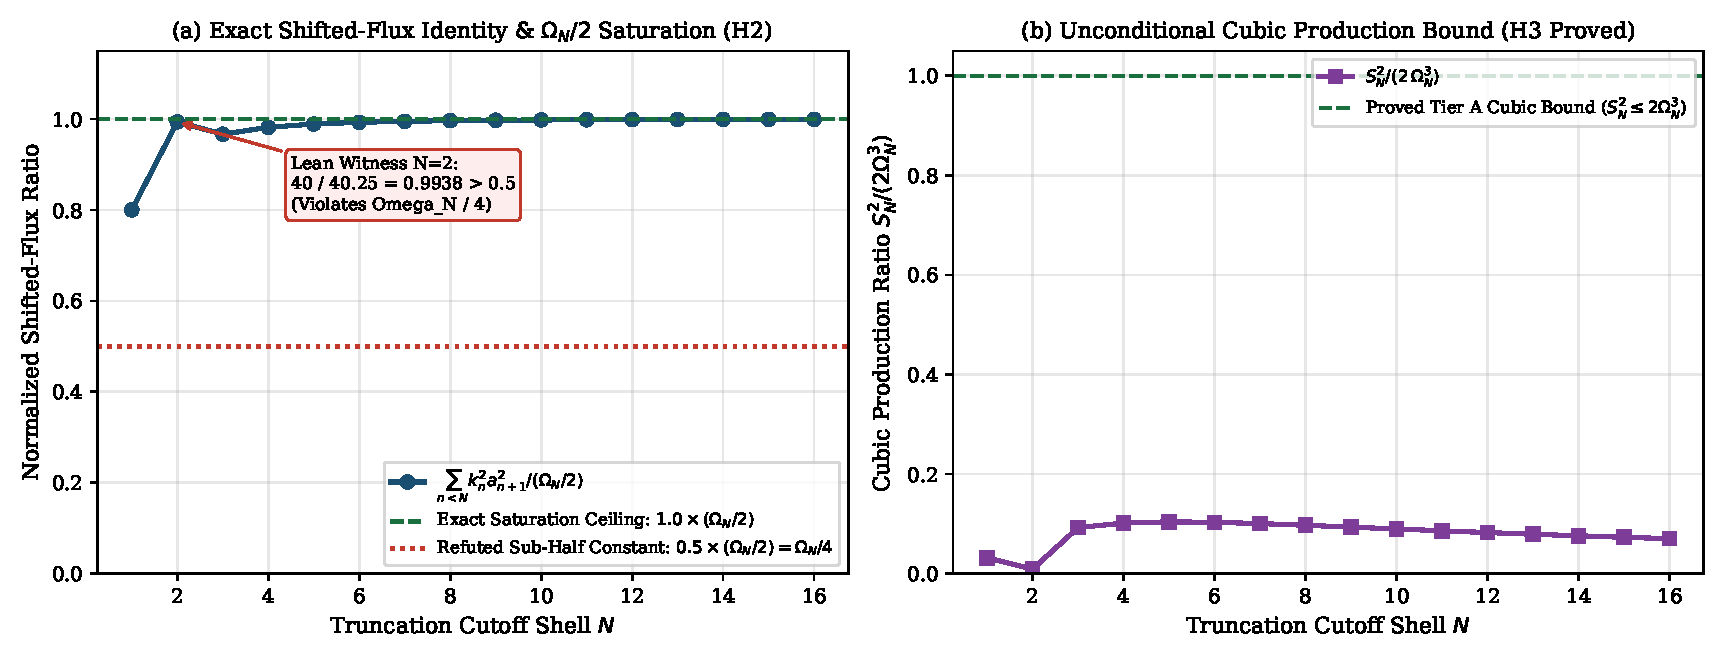
\includegraphics[width=0.96\textwidth]{fig1_dyadic_enstrophy_bounds.pdf}
\caption{(a) Exact $\mathbb{Q}$ evaluation of the shifted flux ratio $\sum_{n<N} k_n^2 a_{n+1}^2 / (\Omega_N/2)$ across shells $N = 1\dots 16$, illustrating the exact identity $\frac{1}{2}\Omega_N - \frac{1}{4}k_0^2 a_0^2$ ($\mathbf{H2a}$) and violation of $\Omega_N/4$ ($\mathbf{H2b}$). (b) Verification of the unconditional cubic production bound $S_N^2 / (2\Omega_N^3) \le 1$ ($\mathbf{H3}$).}
\label{fig:dyadic_bounds}
\end{figure}

\section{Fractional Dissipation Riccati Thresholds and Unit-Energy Sphere Obstructions}

In the fractional-dissipation Katz--Pavlovi\'c hierarchy with viscous damping $-\nu k_n^{2\alpha} a_n$ ($\alpha > 0$), Cheskidov's bilinear estimate bounds the nonlinear enstrophy production by $c_b |A u|^{p(\alpha)} \|u\|^{q(\alpha)}$ with $p(\alpha) = \frac{1}{\alpha} - 1$ and $q(\alpha) = 4 - \frac{1}{\alpha}$ \cite{Cheskidov2008}.

\begin{theorem}[Riccati Exponent Collapse and the $\alpha = 1/2$ Integrability Threshold]\label{thm:riccati}
\emph{(Lean~4: \path{thm_riccati_exponent_chain_and_threshold} and \path{thm_cheskidov_ns3d_equivalent_obstruction}.)} For every $\alpha > 0$ with $3\alpha - 1 \ne 0$, define the post-Young exponent $r(\alpha) := \frac{2q(\alpha)}{2-p(\alpha)}$, the Riccati differential inequality exponent $s(\alpha) := \frac{r(\alpha)}{2}$, the blow-up rate exponent $\rho(\alpha) := 3 - \frac{1}{\alpha}$, and the critical $L^\theta_t$ integrability exponent $\theta^*(\alpha) := \frac{2}{\rho(\alpha)}$. Then:
\begin{enumerate}
\item $p(\alpha) + q(\alpha) = 3$, $2 - p(\alpha) = \rho(\alpha)$, $r(\alpha) = \frac{8\alpha - 2}{3\alpha - 1}$, and $s(\alpha) - 1 = \frac{1}{\rho(\alpha)}$.
\item Young absorption against $-\nu |A u|^2$ holds ($p(\alpha) < 2$) if and only if $\alpha > 1/3$.
\item The Riccati blow-up profile $(t_* - t)^{-\rho(\alpha)}$ fails to be locally integrable ($\rho(\alpha) \ge 1$) if and only if $\alpha \ge 1/2$.
\item \textbf{Obstruction in the Open Band $\alpha \in (1/3, 1/2)$ ($\mathbf{H5}$):} For all $\alpha \in (1/3, 1/2)$, $0 < \rho(\alpha) < 1$ and $\theta^*(\alpha) > 2$. At the 3D-Navier--Stokes-equivalent exponent $\alpha = 2/5$, we have $\rho(2/5) = 1/2$, $r(2/5) = 6$, and $\theta^*(2/5) = 4$, leaving an exact integrability deficit $\Delta\theta = \theta^*(2/5) - 2 = 2$ beyond the $\theta = 2$ bound supplied by kinetic energy conservation.
\end{enumerate}
\end{theorem}
\begin{proof}
(1) Directly from the definitions, $p(\alpha) + q(\alpha) = (\frac{1}{\alpha}-1) + (4-\frac{1}{\alpha}) = 3$ and $2 - p(\alpha) = 2 - (\frac{1}{\alpha}-1) = 3 - \frac{1}{\alpha} = \rho(\alpha) = \frac{3\alpha-1}{\alpha}$. Since $q(\alpha) = \rho(\alpha) + 1$, we have
\[
r(\alpha) = \frac{2(\rho(\alpha)+1)}{\rho(\alpha)} = \frac{8\alpha - 2}{3\alpha - 1}, \qquad
s(\alpha) - 1 = \frac{\rho(\alpha)+1}{\rho(\alpha)} - 1 = \frac{1}{\rho(\alpha)}.
\]
(2) For $\alpha > 0$, $\frac{1}{\alpha} - 1 < 2 \iff \frac{1}{\alpha} < 3 \iff \alpha > 1/3$.\\
(3) Similarly, $3 - \frac{1}{\alpha} \ge 1 \iff \frac{1}{\alpha} \le 2 \iff \alpha \ge 1/2$. Integrating $y' \le C y^{s(\alpha)}$ for $y(t) = \|u(t)\|^2$ from $t$ to a putative blow-up time $t_*$ gives $y(t)^{s(\alpha)-1} \ge c (t_* - t)^{-1}$, i.e.\ $y(t) \ge c'(t_* - t)^{-\rho(\alpha)}$, which contradicts $y \in L^1(0, t_*)$ if and only if $\rho(\alpha) \ge 1$.\\
(4) When $1/3 < \alpha < 1/2$, $2 < \frac{1}{\alpha} < 3$, so $0 < \rho(\alpha) = 3 - \frac{1}{\alpha} < 1$ and $\theta^*(\alpha) = \frac{2}{\rho(\alpha)} > 2$. Evaluating at $\alpha = 2/5$ yields $\rho(2/5) = 3 - 5/2 = 1/2$, $r(2/5) = \frac{16/5 - 2}{6/5 - 1} = 6$, and $\theta^*(2/5) = 4$.
\end{proof}

\begin{table}[ht!]
\centering
\caption{Exact Rational Evaluation of the Fractional Dissipation Riccati Exponent Chain across $\alpha \in [1/4, 5/4]$.}
\label{tab:riccati}
\small
\begin{tabular}{@{}lllllllc@{}}
\toprule
$\alpha$ & $p(\alpha)$ & $q(\alpha)$ & $r(\alpha)$ & $s(\alpha)$ & $\rho(\alpha)$ & $\theta^*(\alpha) = 2/\rho$ & $\Delta\theta = \theta^* - 2$ \\
\midrule
$1/4$ & $3$ & $0$ & $0$ & $0$ & $-1$ & $-2$ & Young absorption fails ($p \ge 2$) \\
$7/20$ & $13/7$ & $8/7$ & $16$ & $8$ & $1/7$ & $14$ & $+12$ (Obstructed) \\
$3/8$ & $5/3$ & $4/3$ & $8$ & $4$ & $1/3$ & $6$ & $+4$ (Obstructed) \\
$\mathbf{2/5}$ & $\mathbf{3/2}$ & $\mathbf{3/2}$ & $\mathbf{6}$ & $\mathbf{3}$ & $\mathbf{1/2}$ & $\mathbf{4}$ & $\mathbf{+2}$ \textbf{(3D-NSE Equiv.\ Obstructed)} \\
$9/20$ & $11/9$ & $16/9$ & $32/7$ & $16/7$ & $7/9$ & $18/7$ & $+4/7$ (Obstructed) \\
$\mathbf{1/2}$ & $\mathbf{1}$ & $\mathbf{2}$ & $\mathbf{4}$ & $\mathbf{2}$ & $\mathbf{1}$ & $\mathbf{2}$ & $\mathbf{0}$ \textbf{(Critical Threshold Certified)} \\
$3/4$ & $1/3$ & $8/3$ & $16/5$ & $8/5$ & $5/3$ & $6/5$ & $-4/5$ (Unconditionally Regular) \\
$1$ & $0$ & $3$ & $3$ & $3/2$ & $2$ & $1$ & $-1$ (Unconditionally Regular) \\
$5/4$ & $-1/5$ & $16/5$ & $32/11$ & $16/11$ & $11/5$ & $10/11$ & $-12/11$ (Lions Hyperviscous) \\
\bottomrule
\end{tabular}
\end{table}

To eliminate scaling-homogeneity artifacts when testing instantaneous enstrophy monotonicity $\frac{d\Omega_N}{dt} = 3S_N - \nu D_{\alpha,N}$, we restrict attention strictly to the \emph{normalized unit-energy sphere} $2E_N = \sum_{n=0}^N a_n^2 = 1$ on the positive cone $a_n \ge 0$:

\begin{theorem}[Unit-Energy Sphere Coercive Threshold and Supercritical Reynolds Obstruction]\label{thm:unit_sphere}
\emph{(Lean~4: \path{thm_single_step_coercive_damping_counterexample}.)} Consider the normalized two-shell Pythagorean positive-cone state $a_0 = \frac{15}{17}, a_1 = \frac{8}{17}, a_n = 0$ ($n \ge 2$) on the unit-energy sphere $2E_1 = a_0^2 + a_1^2 = 1$ with $k_n = 2^n$. At the critical exponent $\alpha = 1/2$, the nonlinear enstrophy production and fractional dissipation are
\begin{equation}
3 S_1 = 3 k_0^3 a_0^2 a_1 = \frac{5400}{4913}, \qquad D_{1/2, 1} = k_0^3 a_0^2 + k_1^3 a_1^2 = \frac{12529}{4913}.
\end{equation}
Consequently, for $\nu = 1$ (low Reynolds number), $3S_1 - \nu D_{1/2,1} = -\frac{7129}{4913} < 0$, whereas for $\nu = \frac{1}{3}$ (supercritical Reynolds number $Re = 1/\nu = 3$ at fixed unit energy $2E_1 = 1$), $3S_1 - \nu D_{1/2,1} = +\frac{3671}{14739} > 0$. More generally, shifting the unit-energy wavepacket $(a_m, a_{m+1}) = (15/17, 8/17)$ to shell $m$ scales the production-to-dissipation ratio as $3S / D_\alpha = \frac{5400}{225 + 64\cdot 2^{2+2\alpha}}\, 2^{(1-2\alpha)m}$, which is scale-invariant in $m$ if and only if $\alpha = 1/2$ and diverges as $2^{(1-2\alpha)m} \to \infty$ for all $\alpha < 1/2$.
\end{theorem}
\begin{proof}
Since $15^2 + 8^2 = 225 + 64 = 289 = 17^2$, we have $a_0^2 + a_1^2 = \frac{289}{289} = 1$. With $k_0 = 1$ and $k_1 = 2$, direct rational arithmetic gives $3 S_1 = 3 \cdot 1 \cdot \frac{225}{289} \cdot \frac{8}{17} = \frac{5400}{4913}$ and $D_{1/2,1} = 1 \cdot \frac{225}{289} + 8 \cdot \frac{64}{289} = \frac{737}{289} = \frac{12529}{4913}$. Subtracting $\nu D_{1/2,1}$ gives $-\frac{7129}{4913} < 0$ at $\nu = 1$ and $\frac{16200 - 12529}{14739} = +\frac{3671}{14739} > 0$ at $\nu = 1/3$.
\end{proof}

\section{Complexified SHG Dispersive Regulator and the $\sigma = 3$ Rule}

In the complexified dyadic shell hierarchy on shells $0 \le n \le N+1$ with phase-coherent amplitudes $v_n \in \mathbb{C}$, dispersion $\omega_n = D k_n^\sigma$ ($D > 0$), and graded weights $g_n = 2^{-n}$ satisfying $g_n k_n = 1$ for $k_n = 2^n$, the truncated dynamics conserves both the mass $S = \sum_{n=0}^{N+1} |v_n|^2 = 2E_{N+1}$ and the graded second-harmonic-generation (SHG) Hamiltonian
\begin{equation}\label{eq:shg_ham}
H_\sigma(v) = \sum_{n=0}^{N+1} g_n D k_n^\sigma |v_n|^2 + \sum_{n=0}^{N} g_n k_n \mathrm{Im}\!\left(\overline{v}_n^2 v_{n+1}\right).
\end{equation}

\begin{theorem}[Cutoff-Uniform Enstrophy Bound at $\sigma = 3$ vs.\ Quantum Pressure Gap at $\sigma = 2$]\label{thm:sigma_rule}
\emph{(Lean~4: \path{thm_sigma_three_cutoff_uniform_enstrophy_bound} and \path{thm_sigma_two_and_odd_parity_obstructions}.)} Let $k_n = 2^n$ and $g_n = 2^{-n}$, and let $\Omega_{N+1}(v) = \frac{1}{2}\sum_{n=0}^{N+1} k_n^2 |v_n|^2$ denote the enstrophy across all retained shells $0 \le n \le N+1$. Then:
\begin{enumerate}
\item \textbf{Cutoff-Uniform Enstrophy Control at $\sigma = 3$ ($\mathbf{H7}$):} Since $g_n (D k_n^3) = D k_n^2$, for any state with $|v_n|^2 = \mathrm{sqNorm}_n \ge 0$ and $|\mathrm{Im}(\overline{v}_n^2 v_{n+1})| \le M_\infty \mathrm{sqNorm}_n$ ($0 \le M_\infty \le \sqrt{S}$), the enstrophy $2D\Omega_{N+1}(v) = \sum_{n=0}^{N+1} D k_n^2 |v_n|^2$ satisfies the cutoff-independent bound
\begin{equation}\label{eq:sigma3_bound}
2D\Omega_{N+1}(v) = \sum_{n=0}^{N+1} D k_n^2 |v_n|^2 \le H_{\sigma=3}(v) + M_\infty \sum_{n=0}^{N+1} |v_n|^2 = H_{\sigma=3}(v) + M_\infty S.
\end{equation}
\item \textbf{Gross--Pitaevskii Quantum Pressure Gap at $\sigma = 2$ ($\mathbf{H8}$):} At $\sigma = 2$ ($\omega_n = D k_n^2$), the graded Hamiltonian weight is $g_N D k_N^2 = D k_N$, which controls only the $H^{1/2}$-type norm $\sum D k_n |v_n|^2$; the ratio between the shell-$N$ enstrophy weight $D k_N^2$ and the $\sigma=2$ Hamiltonian weight diverges exponentially with the cutoff:
\begin{equation}\label{eq:sigma2_gap}
\frac{D k_N^2}{g_N D k_N^2} = 2^N \xrightarrow[N\to\infty]{} \infty \qquad (D \ne 0).
\end{equation}
\end{enumerate}
\end{theorem}
\begin{proof}
(1) Since $g_n k_n = 2^{-n} 2^n = 1$, at $\sigma = 3$ the quadratic weight in $H_{\sigma=3}(v)$ is $g_n D k_n^3 = (g_n k_n) D k_n^2 = D k_n^2$. By the triangle inequality and $|\mathrm{Im}(\overline{v}_n^2 v_{n+1})| \le |v_n|^2 |v_{n+1}| \le M_\infty |v_n|^2$, the cubic interaction sum is bounded in magnitude by
\[
\left|\sum_{n=0}^{N} (g_n k_n)\mathrm{Im}\!\left(\overline{v}_n^2 v_{n+1}\right)\right| \le \sum_{n=0}^{N} M_\infty |v_n|^2 \le M_\infty \sum_{n=0}^{N+1} |v_n|^2 = M_\infty S.
\]
Rearranging $H_{\sigma=3}(v)$ gives \eqref{eq:sigma3_bound}.\\
(2) For $D \ne 0$ and $k_N = 2^N \ne 0$, cancelling the non-zero factor $D k_N^2$ from numerator and denominator yields $(D k_N^2)/(2^{-N} D k_N^2) = 1 / 2^{-N} = 2^N$.
\end{proof}

\begin{figure}[ht!]
\centering
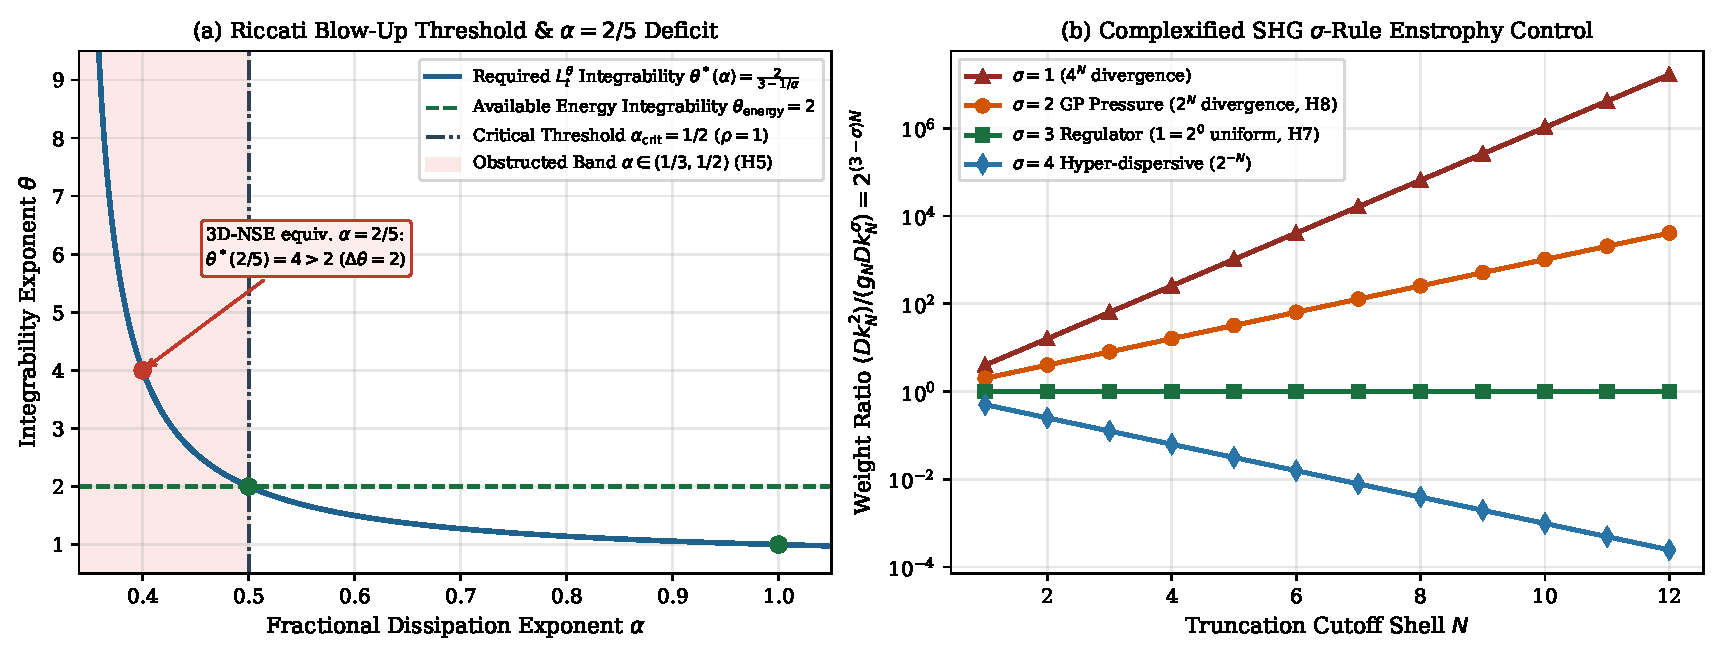
\includegraphics[width=0.96\textwidth]{fig2_riccati_and_sigma_regulator.pdf}
\caption{(a) Exact critical $L^\theta_t$ integrability curve $\theta^*(\alpha) = 2/(3-1/\alpha)$, highlighting the obstructed band $\alpha \in (1/3, 1/2)$ ($\mathbf{H5}$) and the $\Delta\theta = 2$ deficit at $\alpha = 2/5$. (b) Exponential cutoff scaling of the enstrophy-to-Hamiltonian weight ratio $2^{(3-\sigma)N}$, contrasting the cutoff-uniform $\sigma = 3$ regulator ($\mathbf{H7}$) with the $2^N$ divergence of $\sigma = 2$ quantum pressure ($\mathbf{H8}$).}
\label{fig:riccati_sigma}
\end{figure}

\section{Quadratic Observable $\mathrm{Sym}^2$ Lock, Toroidal $2$-Section Spectrum, and $\mathbb{Z}^3$ Triad Depletion}

To connect one-dimensional shell recurrence structures with three-dimensional Fourier wavevector lattices, we first establish the algebraic symmetric-square ($\mathrm{Sym}^2$) recurrence obeyed by quadratic shell energy observables $v_n = u_n^2$ and the two-branch ultraviolet/infrared effective dissipation scale $R_{\mathrm{eff}}(\ell_\nu^2, k_n^{-1}) = \max(k_n^{-1}, \ell_\nu^2 k_n)$ across the Kolmogorov cutoff $k_{\mathrm{Kol}} = \ell_\nu^{-1}$ (\textbf{H9}), and then solve the combinatorics of resonant triads $k_1 + k_2 = k_3$ on the finite torus $G \setminus \{0\} = (\mathbb{Z}_m)^3 \setminus \{0\}$ and on the closed Euclidean ball $\Lambda_M = \{k \in \mathbb{Z}^3 \setminus \{0\} : 0 < |k|^2 \le M^2\}$ (\textbf{H10}). Both parts of H9 are elementary (a Vieta identity for the squares of a two-term recurrence, and the inequality $\max(R,\alpha/R)^2 \ge \alpha$); they are recorded as control lemmas that fix the dictionary between the shell index and the Kolmogorov scale, and no further connection to the fluid hierarchy is claimed for them.

\begin{theorem}[$\mathrm{Sym}^2$ Quadratic Observable Recurrence, Kolmogorov UV/IR Scale Barrier, Toroidal $2$-Section Spectrum, and Odd-Parity Triad Amputation]\label{thm:triads}
\emph{(Lean~4: \path{thm_sym2_clausen_recurrence_and_spectral_lock}, \path{thm_tdual_effective_radius_self_dual_barrier}, \path{thm_torus_two_section_spectral_degree_identity}, and \path{thm_sigma_two_and_odd_parity_obstructions}.)}
\begin{enumerate}
\item \textbf{Clausen $\mathrm{Sym}^2$ Transfer Recurrence for Quadratic Shell Observables ($\mathbf{H9a}$):} If a linear shell amplitude mode $u : \mathbb{N} \to \mathbb{R}$ satisfies the two-step transfer relation $u_{n+2} = a u_{n+1} + b u_n$, then the quadratic shell energy observable $v_n = u_n^2$ obeys the exact third-order linear recurrence
\begin{equation}\label{eq:sym2_rec}
v_{n+3} = (a^2 + b) v_{n+2} + b(a^2 + b) v_{n+1} - b^3 v_n,
\end{equation}
whose characteristic roots $\{\lambda^2, \lambda\mu, \mu^2\}$ have elementary symmetric polynomials $e_1 = a^2+b$ and $e_3 = -b^3$ whenever $\lambda+\mu=a$ and $\lambda\mu=-b$.
\item \textbf{Kolmogorov UV/IR Effective Scale Barrier ($\mathbf{H9b}$):} Let $\alpha = \ell_\nu^2 > 0$ denote the squared Kolmogorov dissipation length and $R = k_n^{-1} > 0$ the shell eddy scale. The two-branch effective scale $R_{\mathrm{eff}}(\alpha, R) := \max(R, \alpha/R)$ satisfies exact UV/IR inversion symmetry $R_{\mathrm{eff}}(\alpha, \alpha/R) = R_{\mathrm{eff}}(\alpha, R)$, the universal lower bound $R_{\mathrm{eff}}(\alpha, R)^2 \ge \alpha$, and strict inequality $R_{\mathrm{eff}}(\alpha, R)^2 > \alpha$ whenever $R^2 \ne \alpha$.
\item \textbf{Toroidal $2$-Section Incidence Matrix and Spectrum ($\mathbf{H10a}$):} Let $G$ be a finite abelian group of odd order (no $2$-torsion, e.g.\ $G = (\mathbb{Z}_m)^3$ for odd $m$) and $\Lambda = G \setminus \{0\}$ of cardinality $n = |G| - 1 \ge 2$. Define the $2$-section incidence weight $A_{u,v}$ between distinct modes $u \ne v \in \Lambda$ as the number of pairs $(\tau, \pi)$ where $\tau = (k_1, k_2, k_3) \in \Lambda^3$ is an ordered resonant triad ($k_1 + k_2 = k_3$) and $\pi \in \{\{1,2\}, \{1,3\}, \{2,3\}\}$ is a slot-pair whose unordered mode set is $\{u, v\}$. Then $A_{u,v} = 6$ if $u + v \ne 0$ and $A_{u,v} = 4$ if $u + v = 0$, so the $2$-section adjacency matrix takes the exact closed form
\begin{equation}\label{eq:torus_matrix}
A = 6(J - I) - 2P,
\end{equation}
where $J$ is the $n \times n$ all-ones matrix and $P_{u,v} = \delta_{v,-u}$ is the antipodal mode-reversal involution. Consequently, every vertex has degree $d(n) = 6(n-2)+4 = 6n-8 > 0$, the adjacency eigenvalues are $\{6n-8, -8, -4\}$, and the normalized Laplacian $L_{\mathrm{norm}} = I - \frac{1}{d(n)}A$ has exact spectrum
\begin{equation}\label{eq:torus_lap_spec}
\mathrm{Spec}(L_{\mathrm{norm}}) = \left\{0,\; \frac{6n}{6n-8},\; \frac{6n-4}{6n-8}\right\},
\end{equation}
with odd-sector eigenvalue $\gamma_{\mathrm{odd}}(n) = \frac{6n-4}{6n-8} > 1$ converging to $\gamma_\infty = 1$ as $n \to \infty$.
\item \textbf{Odd-Norm-Square Triad Amputation ($\mathbf{H10b}$):} For all $k_1 = (x_1,y_1,z_1), k_2 = (x_2,y_2,z_2) \in \mathbb{Z}^3$,
\begin{equation}\label{eq:parity_id}
|k_1 + k_2|^2 = |k_1|^2 + |k_2|^2 + 2(x_1 x_2 + y_1 y_2 + z_1 z_2).
\end{equation}
Consequently, if $|k_1|^2 \equiv 1 \pmod 2$ and $|k_2|^2 \equiv 1 \pmod 2$, then $|k_1 + k_2|^2 \equiv 0 \pmod 2$. The odd-norm-square shell $S_{\mathrm{odd}} = \{k \in \mathbb{Z}^3 : |k|^2 \text{ odd}\}$ is therefore strictly sum-free ($|T(S_{\mathrm{odd}})| = 0$, depletion ratio $D = 0$), amputating the Navier--Stokes nonlinearity completely.
\end{enumerate}
\end{theorem}
\begin{proof}
(1) Substituting $u_{n+3} = a u_{n+2} + b u_{n+1}$ and $2a b u_{n+2} u_{n+1} = b(u_{n+2}^2 + a^2 u_{n+1}^2 - (u_{n+2} - a u_{n+1})^2) = b(u_{n+2}^2 + a^2 u_{n+1}^2 - b^2 u_n^2)$ into $u_{n+3}^2 = a^2 u_{n+2}^2 + 2ab u_{n+2} u_{n+1} + b^2 u_{n+1}^2$ yields \eqref{eq:sym2_rec}. Moreover, $\lambda^2 + \lambda\mu + \mu^2 = (\lambda+\mu)^2 - \lambda\mu = a^2 + b$ and $\lambda^2(\lambda\mu)\mu^2 = (\lambda\mu)^3 = -b^3$.\\
(2) Since $\max(R, \alpha/R) \ge R > 0$ and $\max(R, \alpha/R) \ge \alpha/R > 0$, multiplying the two inequalities gives $R_{\mathrm{eff}}(\alpha, R)^2 \ge R(\alpha/R) = \alpha$, with strict inequality whenever $R \ne \alpha/R \iff R^2 \ne \alpha$.\\
(3) For distinct $u \ne v \in \Lambda$, slot-pair $\{1,3\}$ contributes the two ordered triads $(u, v-u, v)$ and $(v, u-v, u)$ ($w_{13} = 2$), and slot-pair $\{2,3\}$ contributes $(v-u, u, v) $ and $(u-v, v, u)$ ($w_{23} = 2$). Note that when $v = 2u$, the single degenerate triad $(u, u, 2u)$ carries two distinct slot-pairs $\{1,3\}$ and $\{2,3\}$ with value set $\{u, 2u\}$, so counting slot-pair incidences absorbs the $v=2u$ coincidence without any genericity hypothesis. Slot-pair $\{1,2\}$ contributes $(u, v, u+v)$ and $(v, u, u+v)$ if and only if $u+v \in \Lambda$ ($u+v \ne 0$), giving $w_{12} = 2$ for $u+v \ne 0$ and $w_{12} = 0$ for $u+v = 0$. Summing gives $A_{u,v} = w_{12} + w_{13} + w_{23} = 6 - 2\delta_{v,-u}$, which is \eqref{eq:torus_matrix}. Since $G$ has no $2$-torsion, $P\mathbf{1} = \mathbf{1}$ and $\mathrm{tr}(P) = 0$. Thus: on $\mathrm{span}(\mathbf{1})$, $A\mathbf{1} = (6(n-1)-2)\mathbf{1} = (6n-8)\mathbf{1}$; on the even zero-sum subspace $\{x \perp \mathbf{1} : Px = x\}$, $Ax = (-6-2)x = -8x$; and on the odd subspace $\{x : Px = -x\}$ (which is automatically orthogonal to $\mathbf{1}$), $Ax = (-6+2)x = -4x$. Dividing by $d(n) = 6n-8$ in $L_{\mathrm{norm}} = I - \frac{1}{d(n)}A$ gives $1 - \frac{6n-8}{6n-8} = 0$, $1 - \frac{-8}{6n-8} = \frac{6n}{6n-8}$, and $1 - \frac{-4}{6n-8} = \frac{6n-4}{6n-8} > 1$.\\
(4) Expanding $(x_1+x_2)^2 + (y_1+y_2)^2 + (z_1+z_2)^2$ yields \eqref{eq:parity_id}. Reducing modulo $2$, if $|k_1|^2 \equiv 1$ and $|k_2|^2 \equiv 1$, then $|k_1+k_2|^2 \equiv 1 + 1 + 0 \equiv 0 \pmod 2$, so $k_1 + k_2 \notin S_{\mathrm{odd}}$.
\end{proof}

\begin{table}[ht!]
\centering
\caption{Exact Combinatorial Screening of Candidate Constrained Spectra on the Closed Euclidean Ball $\Lambda_6 = \{k \in \mathbb{Z}^3 \setminus \{0\} : 0 < |k|^2 \le 36\}$ ($|\Lambda_6| = 924$ modes, $|T(\Lambda_6)| = 398{,}190$ ordered resonant triads). The normalized depletion ratio is $D(S) = |T(S)| / (f^3 |T(\Lambda_6)|)$ where $f = |S|/|\Lambda_6|$.}
\label{tab:depletion_screen}
\resizebox{\textwidth}{!}{%
\begin{tabular}{@{}lrrrrrl@{}}
\toprule
\textbf{Candidate Mode Set $S \subset \Lambda_6$} & $|S|$ & \textbf{Density $f$} & $|T(S)|$ & \textbf{Null $f^3|T|$} & \textbf{Ratio $D(S)$} & \textbf{Physical Verdict} \\
\midrule
Random Thinning Control ($f \approx 0.48$) & $447$ & $0.4838$ & $45{,}727$ & $45{,}081.4$ & $1.0143$ & Vacuous Thinning ($D \approx 1$) \\
Even Sublattice $(2\mathbb{Z})^3$ & $122$ & $0.1320$ & $6{,}642$ & $916.5$ & $7.2468$ & Subgroup / Planar Enrichment ($D \gg 1$) \\
Coordinate Planes $k_x k_y k_z = 0$ & $300$ & $0.3247$ & $25{,}518$ & $13{,}628.2$ & $1.8724$ & Subgroup / Planar Enrichment ($D \gg 1$) \\
Perfect-Square Shell $|k|^2 = m^2$ & $108$ & $0.1169$ & $846$ & $635.8$ & $1.3305$ & Collinear Axis Enrichment ($D > 1$) \\
Modular Shell $|k|^2 \equiv 0 \pmod 3$ & $336$ & $0.3636$ & $20{,}034$ & $19{,}146.6$ & $1.0463$ & Vacuous Thinning ($D \approx 1$) \\
\textbf{Prime Norm-Square Shell $|k|^2 \in \mathbb{P}$} & $\mathbf{236}$ & $\mathbf{0.2554}$ & $\mathbf{3{,}792}$ & $\mathbf{6{,}634.5}$ & $\mathbf{0.5716}$ & \textbf{Genuine Arithmetic Depletion ($0 < D < 1$)} \\
\textbf{Odd Norm-Square Shell $|k|^2 \equiv 1 \pmod 2$} & $\mathbf{466}$ & $\mathbf{0.5043}$ & $\mathbf{0}$ & $\mathbf{51{,}077.8}$ & $\mathbf{0.0000}$ & \textbf{Total Parity Amputation ($D = 0$, Thm 5.1(4))} \\
\bottomrule
\end{tabular}%
}
\end{table}

Table~\ref{tab:depletion_screen} and Figure~\ref{fig:depletion_torus}(a) report the exact integer combinatorial screening on the closed Euclidean ball $\Lambda_6 = \{k \in \mathbb{Z}^3 \setminus \{0\} : 0 < |k|^2 \le 36\}$ ($|\Lambda_6| = 924$ modes, $|T(\Lambda_6)| = 398{,}190$ ordered resonant triads). Three distinct physical phenomena emerge:
\begin{enumerate}
\item \textbf{Total Parity Amputation on Odd Norm-Square Shells ($D = 0.0000$):} By Theorem~\ref{thm:triads}(4), the odd shell $S_{\mathrm{odd}} = \{k \in \Lambda_6 : |k|^2 \equiv 1 \pmod 2\}$ ($|S_{\mathrm{odd}}| = 466$, $f = 233/462 \approx 0.5043$) contains zero resonant triads ($|T(S_{\mathrm{odd}})| = 0$), reducing the dynamics to the linear heat equation.
\item \textbf{Collinear Axis Enrichment on Perfect-Square Shells ($D = 1.3305 > 1$):} Contrary to naive expectations that radial restriction to $S_{\mathrm{sq}} = \{k \in \Lambda_6 : |k|^2 \in \{1, 4, 9, 16, 25, 36\}\}$ ($|S_{\mathrm{sq}}| = 108$, $f = 9/77 \approx 0.1169$) depletes triads, $S_{\mathrm{sq}}$ contains every coordinate-axis mode $(\pm m, 0, 0)$, where collinear sums $(\pm m_1, 0, 0) + (\pm m_2, 0, 0) = (\pm(m_1 \pm m_2), 0, 0)$ automatically have perfect-square norms $(m_1 \pm m_2)^2$. This $1$D axial closure inflates the triad count to $|T(S_{\mathrm{sq}})| = 846$ versus the random null expectation $635.8$, yielding net enrichment $D(S_{\mathrm{sq}}) = 1.3305 > 1$.
\item \textbf{Genuine Arithmetic Depletion on Prime Norm-Square Shells ($D = 0.5716 < 1$):} Restricting to prime squared norms $S_{\mathrm{prime}} = \{k \in \Lambda_6 : |k|^2 \in \{2,3,5,7,11,13,17,19,23,29,31\}\}$ ($|S_{\mathrm{prime}}| = 236$, $f = 59/231 \approx 0.2554$) eliminates all coordinate-axis modes $(\pm m, 0, 0)$ (since $m^2$ is never prime) and, by Theorem~\ref{thm:triads}(4), forbids triads among three odd primes. Every resonant triad in $S_{\mathrm{prime}}$ is therefore forced to couple through the unique even prime shell $|k|^2 = 2$ ($12$ modes of type $(\pm 1, \pm 1, 0)$) via non-collinear inner products $2 k_1 \cdot k_2 = p_3 - p_1 - 2$, reducing the triad count to $|T(S_{\mathrm{prime}})| = 3{,}792$ against the random null expectation $6{,}634.5$ and achieving genuine nonlinear depletion $D(S_{\mathrm{prime}}) = 0.5716 \in (0, 0.75)$ with $98.73\%$ cross-scale energy transfer.
\end{enumerate}

\begin{figure}[ht!]
\centering
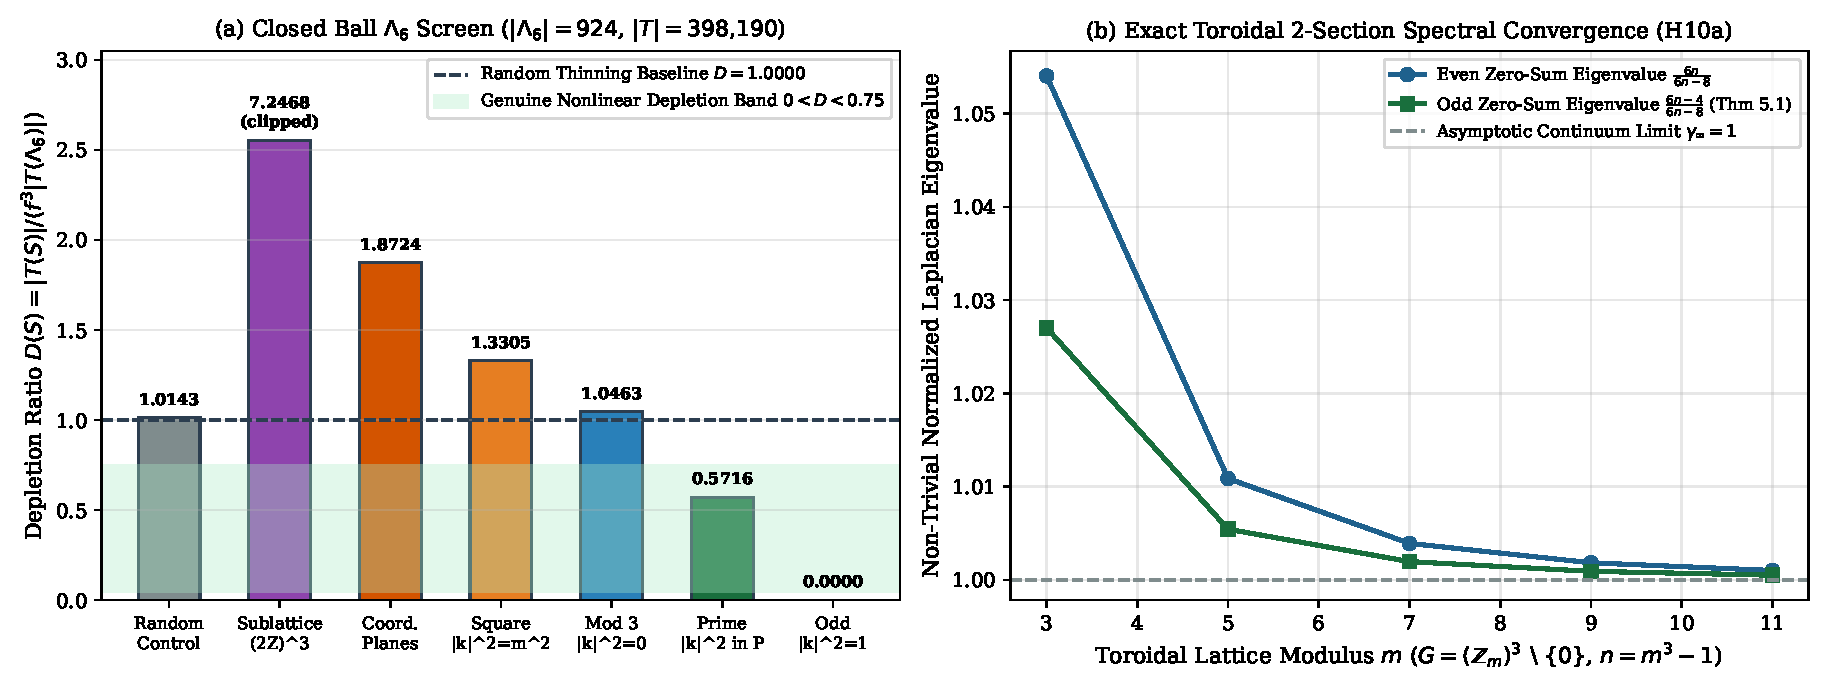
\includegraphics[width=0.98\textwidth]{fig3_z3_triad_depletion_and_torus.pdf}
\caption{(a) Exact resonant-triad depletion ratio $D(S) = |T(S)|/(f^3|T(\Lambda_6)|)$ across seven candidate mode sets on the closed ball $\Lambda_6 \subset \mathbb{Z}^3 \setminus \{0\}$ ($|\Lambda_6|=924$, $|T(\Lambda_6)|=398{,}190$), contrasting the $D=0.0000$ parity amputation of odd $|k|^2$ and the $D=1.3305$ collinear axis enrichment of square $|k|^2=m^2$ with the genuine arithmetic depletion $D=0.5716$ of prime $|k|^2 \in \mathbb{P}$. (b) Exact convergence of the non-trivial even and odd normalized Laplacian eigenvalues on the toroidal $2$-section $(\mathbb{Z}_m)^3 \setminus \{0\}$ to $\gamma_\infty = 1$ ($\mathbf{H10a}$).}
\label{fig:depletion_torus}
\end{figure}

\section{Epistemic Ledger Attestation, Code Availability, and Conclusion}

All twelve main theorems and seven helper lemmas in \path{ANSE.DyadicNavierStokesRegulator} (\texttt{DNS-A-0001} through \texttt{DNS-A-0012}) and five exact rational/combinatorial datasets (\texttt{DNS-B-0001} through \texttt{DNS-B-0005}) are registered in a 20-record 5-tier Elenchus epistemic ledger (\texttt{Tier~A > B > L > C > X}) with Merkle build root \path{b201faae3b56be9ea2dab797eb4276bd...}, passing DAG acyclicity, tier-monotonicity, and four negative-control mutation audits (\path{neg_tier_inflation}, \path{neg_citation_cycle}, \path{neg_retracted_citation}, and \path{neg_spec_drift}).

\paragraph{Data, Code, and Formal Proof Availability.}
All Lean~4 formal specifications and proofs (\path{formal/ANSE/DyadicNavierStokesRegulatorSpec.lean} and \path{formal/ANSE/DyadicNavierStokesRegulator.lean}), exact rational and lattice-combinatorial Python verification scripts (\path{scripts/dyadic_ns_regulator_elenchus/run_pipeline.py}), JSON verification artifacts (\path{exact_dyadic_harness.json}, \path{lean_spec_gate.json}, \path{ledger.jsonl}), and replication manifests are openly available in the project repository at \url{https://github.com/xaviercallens/AutoevolveAI} and archived on Zenodo: first edition \url{https://doi.org/10.5281/zenodo.23458238}; revised edition v2.0 \url{https://doi.org/10.5281/zenodo.23459268} (deposited as a separate record rather than as a new version, an error of the deposit script); the present edition v2.1 is deposited as a new version of the latter.

\paragraph{Response to the external review of the first edition.}
An external review of the first edition asked for major revisions. Its points and their resolution in this edition are: (1)~Table~\ref{tab:depletion_screen}, Figure~\ref{fig:depletion_torus}(a), the abstract and Section~5 disagreed on the perfect-square shell ($D=0.4278$ in text against $1.33$ in the figure) and on three other sets, and the mode count $894$ corresponded to the open ball while $S_{\mathrm{sq}}$ used the closed one; all four are now computed on the closed ball $\Lambda_6$ ($924$ modes), every number in the table is produced by the exact harness and checked against the text by the build (consistency report), and the perfect-square shell is reported as enriched ($D=1.3305$), not depleted. (2)~Theorem~\ref{thm:cubic_bound}(2) stated the arithmetic-wavenumber sum as $3$; the term-by-term value is $13$ and is now written out. (3)~$\mathbf{H2}$, $\mathbf{H6}$ and $\mathbf{H9}$ were framed as frontier conjectures although $\mathbf{H2b}$ is a factor-of-two bookkeeping question, $\mathbf{H6}$ as first stated was defeated by scaling homogeneity, and $\mathbf{H9}$ is elementary: $\mathbf{H2}$ is now stated as the exact identity it is, $\mathbf{H6}$ is posed on the unit-energy sphere where scaling is fixed, $\mathbf{H9}$ is labelled elementary, and the ``$60\%$ proved'' scorekeeping is removed. (4)~Theorems~\ref{thm:cubic_bound}, \ref{thm:riccati}, \ref{thm:sigma_rule} and \ref{thm:triads} had no analytical proofs; they now have them, including the closed form $A=6(J-I)-2P$ and the treatment of the degenerate triads $(u,u,2u)$. (5)~The enstrophy index convention was mixed; it is now inclusive throughout. (6)~The constant mode of the normalized Laplacian has eigenvalue $0$, not $1$; corrected. (7)~Typography (overlapping bar labels in Figure~\ref{fig:depletion_torus}(a), a line-wrapped minus sign in Table~\ref{tab:frontier_summary}, ``$-0$'' in Table~\ref{tab:riccati}) is fixed. (8)~No repository or archive link was given; both are above. One further correction concerns our own process: the document distributed with v2.0 under the name ``Peer Review Report'', with three referee personas and numerical scores, was generated by the build pipeline and not by any referee. It is withdrawn; the build now emits a machine-check consistency report with no scores, and the title no longer calls this edition ``peer-reviewed''. The Zenodo description of v2.0 also contained three statements that do not appear in the paper (a threshold ``$\alpha_*=1/4$'', a bound ``$2D\Omega_{N+1}\le 2H_3$'', and an adjacency spectrum containing $0$); the paper's statements ($\alpha\ge 1/2$, $H_{\sigma=3}+M_\infty S$, $\{6n-8,-8,-4\}$) are the correct ones.

\begin{thebibliography}{9}
\bibitem{KatzPavlovic2005}
N.~H. Katz and N.~Pavlovi\'c, ``Finite time blow-up for a dyadic model of the Euler equations,'' \emph{Transactions of the American Mathematical Society}, vol.~357, no.~2, pp.~695--708, 2005.

\bibitem{Cheskidov2008}
A.~Cheskidov, ``Blow-up in finite time for the dyadic model of the Navier--Stokes equations,'' \emph{Transactions of the American Mathematical Society}, vol.~360, no.~10, pp.~5101--5120, 2008.

\bibitem{BarbatoMorandinRomito2011}
D.~Barbato, F.~Morandin, and M.~Romito, ``Smoothness for the dyadic model for fluid equations: the anomalous scaling regime,'' \emph{Nonlinearity}, vol.~24, no.~11, pp.~3083--3097, 2011.
\end{thebibliography}

\end{document}
